

%%%%%%%%%%%%%%%%%%%%%%%%%%%%%%%%%%%%%%%%%%%%%%%%%%%%%%%%%%%%%%%%%%%%%%

\begin{frame}[plain,label=CeSb2Grouplist]
    \frametitle {\mbox{Superconductivity beyond the Pauli limit in high-pressure CeSb2}}
    \includegraphics[width=1.2\textwidth]{\data/CeSb2/FiguresCeSb2/Collaborators/CeSb2CollaboratorsBlue.pdf}
    %\vspace{0 em}
    %\centerline{\makebox[\linewidth]{\rule{0.85\textwidth}{0.4pt}}}
    %%\centerline{\scriptsize L. Klintberg Phys. Rev. Lett. {\bf 109,} 237008 (2012), S. Goh Phys. Rev. Lett. {\bf 114,} 097002 (2015)}
    % \centerline{\scriptsize O. Squire (2022), C. de Podesta (2022)}
    \vfill
\centerline{\makebox[\linewidth]{\rule{0.85\textwidth}{0.4pt}}}

\centerline{\scriptsize Squire PRL {\bf 131,} 026001 (2023), de Podesta (2023)}

\end{frame}
    
%%%%%%%%%%%%%%%%%%%%%%%%%%%%%%%%%%%%%%%%%%%%%%%%%%%%%%%%%%%%%%%%%%%%%%
%\begin{frame}[plain,label=TitlePage]
\begin{frame}
%\centerline{\multiinclude[<visible@+-| +->][format=pdf,graphics={width=\columnwidth}]{\Figures/FermInstab/QPTScenariosHostGuest2}}
\centerline{ 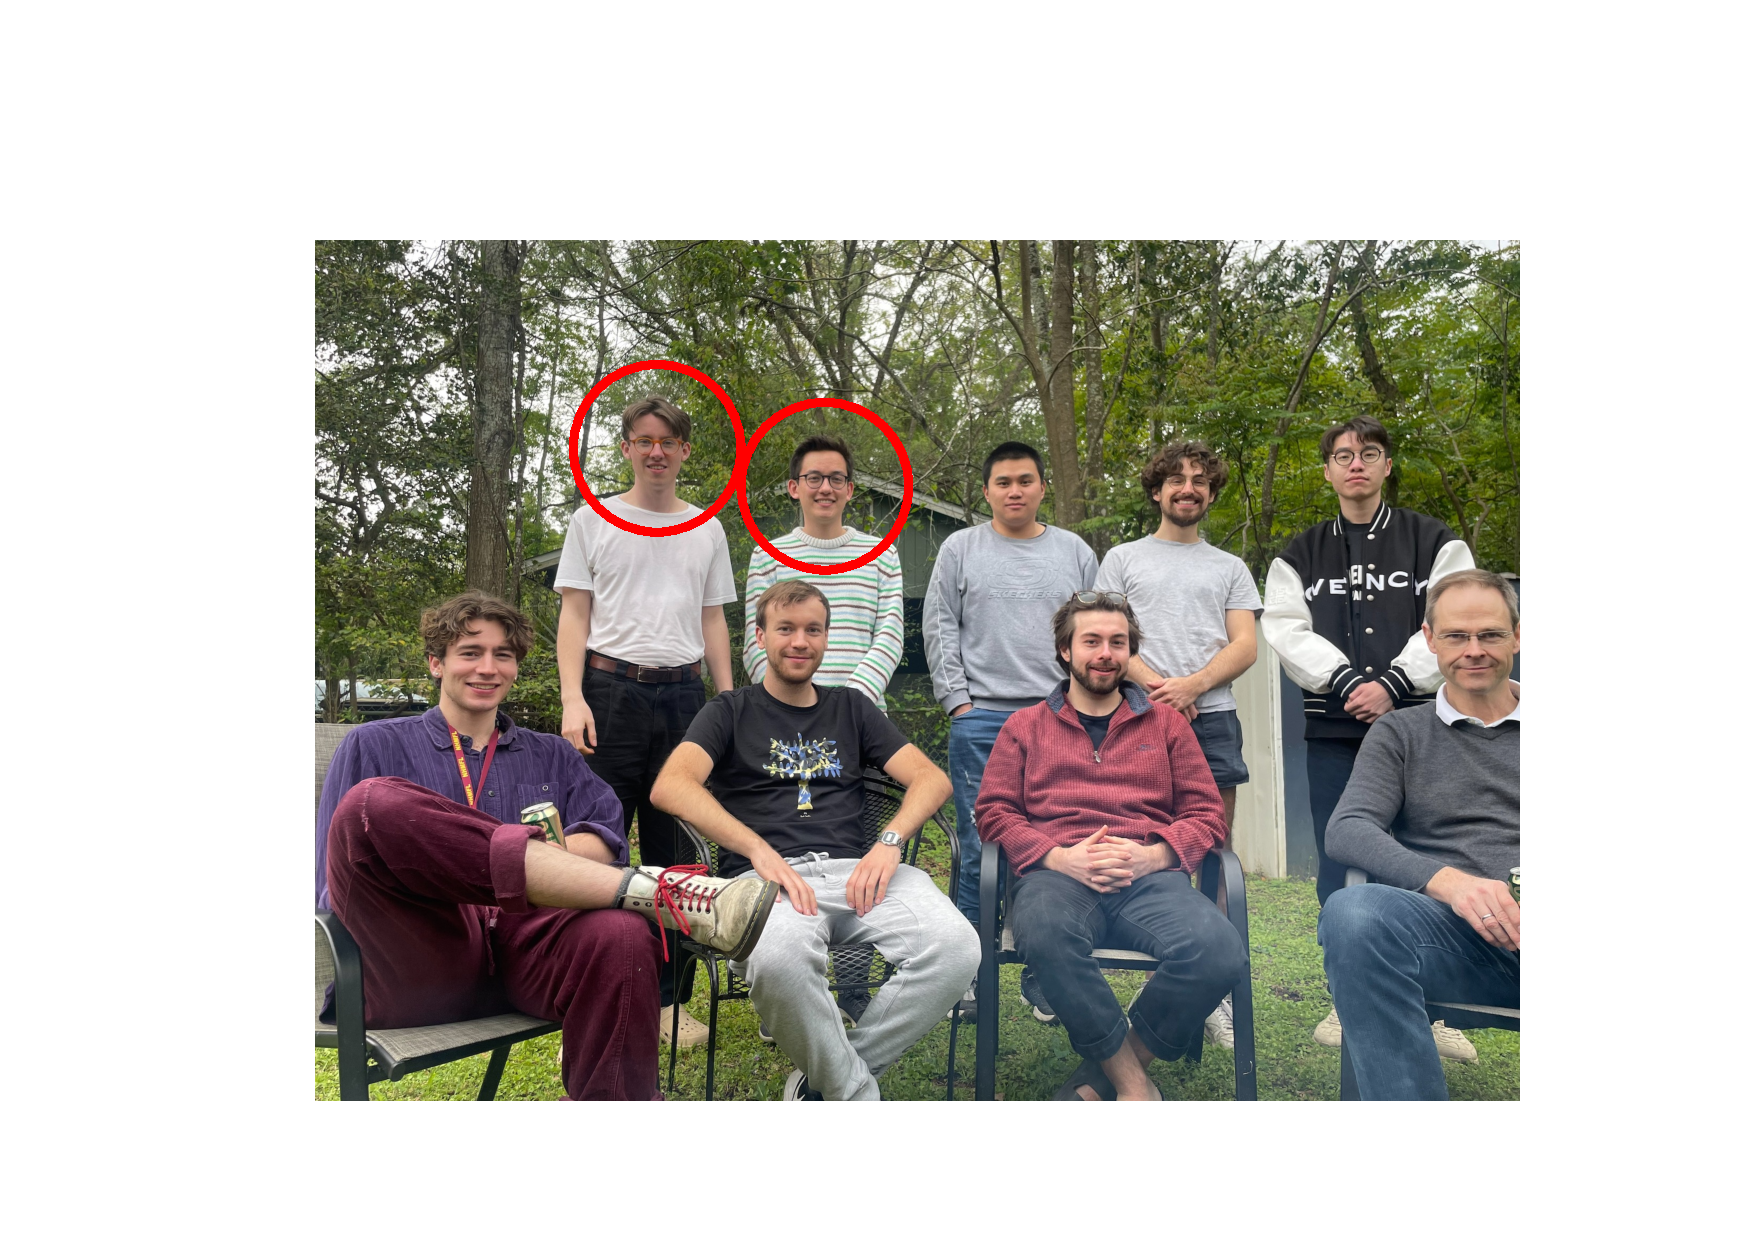
\includegraphics[width=\columnwidth]{GroupPhoto}}

\centerline{\small Cavendish spring expedition to NHMFL Tallahassee}

\vspace{0em}
\centerline{\makebox[\linewidth]{\rule{0.85\textwidth}{0.4pt}}}
%\centerline{\scriptsize L. Klintberg Phys. Rev. Lett. {\bf 109,} 237008 (2012), S. Goh Phys. Rev. Lett. {\bf 114,} 097002 (2015)}

\centerline{\scriptsize Squire PRL {\bf 131,} 026001 (2023), de Podesta (2023)}

\end{frame}
        

%%%%%%%%%%%%%%%%%%%%%%%%%%%%%%%%%%%%%%%%%%%%%%%%%%%%%%%%%%%%%%%%%%%%%%
%\section{CeSb$_2$ Structure}

\subsection{FM Kondo lattice at $p=0$}
%%%%%%%%%%%%%%%%%%%%%%%%%%%%%%%%%%%%%%%%%%%%%%%%%%%%%%%%%%%%%%%%%%%%%%
\begin{frame}[label=CeSb2Intro]
\frametitle{Ferromagnetic Kondo lattice CeSb$_2$}
\centerline{\includegraphics[width=\columnwidth]{\data/CeSb2/FiguresCeSb2/OverviewMagnetic}}

\vspace{1.5em}
\begin{itemize}
\item Orthorhombic structure, same as LaSb$_2$, SmSb$_2$.

\item Reported ferromagnetic below $T_c \simeq 15~\rm K$, at least two more low-$T$ transitions.
%
%\item Ferromagnetism disappears at moderate $p_c \simeq 20~{\rm kbar}$.
%\item Can we observe a ferromagnetic qcp?
\end{itemize}

\vspace{3 em}
\centerline{\makebox[\linewidth]{\rule{0.85\textwidth}{0.4pt}}}

\centerline{\scriptsize Bud'ko PRB {\bf 57} 13624 (1998)}
\end{frame}


\subsection{High-$p$ structural change}
%%%%%%%%%%%%%%%%%%%%%%%%%%%%%%%%%%%%%%%%%%%%%%%%%%%%%%%%%%%%%%%%%%%%%%
\begin{frame}[label=CeSb2Res]
\frametitle{High pressure resistivity in CeSb$_2$}
\vspace{0em}
%\centerline{\multiinclude[<+- | visible@+>] [graphics={width=\columnwidth},format=pdf]{\data/CeSb2/FiguresCeSb2/p30b/CeSb2RTmagn} }
\centerline{\multiinclude[<+- | visible@+>] [graphics={width=0.8\columnwidth},format=pdf]{\data/CeSb2/FiguresCeSb2/HighTHighPResist/CeSb2StructTransFig}}

\vspace{0em}
\begin{itemize}
\item <visible@1-> Low $T$ magnetic transitions.

\item <visible@2-> Transitions shift little initially, then abrupt change.

%\item <visible@3-> Hysteresis at high temperature, moving to lower $T$.

\item <visible@3-> Strong hysteresis. Pressure-induced structural transition?!
\end{itemize}

\end{frame}



\subsection{Structure resolution}

%%%%%%%%%%%%%%%%%%%%%%%%%%%%%%%%%%%%%%%%%%%%%%%%%%%%%%%%%%%%%%%%%%%%%%
\begin{frame}[label=CeSb2xray-0]
\frametitle{High pressure x-ray diffration in CeSb$_2$}
\centerline{\includegraphics[width=\columnwidth]{\data/CeSb2/FiguresCeSb2/DLS2022/PatternsFig}}

\vspace{0em}
\centerline{\makebox[\linewidth]{\rule{0.85\textwidth}{0.4pt}}}
\centerline{\scriptsize C. de Podesta, T. Weinberger, C. Beavers, Diamond Light Source 2022}


\end{frame}


%%%%%%%%%%%%%%%%%%%%%%%%%%%%%%%%%%%%%%%%%%%%%%%%%%%%%%%%%%%%%%%%%%%%%%
\begin{frame}[label=CeSb2xray-1]
\frametitle{RSb$_2$ structures, Lanthanide contraction}
\centerline{\includegraphics[width=0.75\columnwidth]{\data/CeSb2/FiguresCeSb2/DLS2022/StructureTypes}}

\end{frame}


%%%%%%%%%%%%%%%%%%%%%%%%%%%%%%%%%%%%%%%%%%%%%%%%%%%%%%%%%%%%%%%%%%%%%%
\begin{frame}[label=CeSb2muSR]
    \frametitle{High pressure muSR in CeSb$_2$}
    \vspace{0em}
    \centerline{\includegraphics[width=\columnwidth]{\data/CeSb2/FiguresCeSb2/muSR/muSRSummary}}
    
    \begin{itemize}
    \item Zero-field asymmetry signal suggests magnetic order.
    \item Probably incommensurate SDW.
    \end{itemize}
    
    
    \vspace{0em}
    \centerline{\makebox[\linewidth]{\rule{0.85\textwidth}{0.4pt}}}
    %\centerline{\scriptsize L. Klintberg Phys. Rev. Lett. {\bf 109,} 237008 (2012), S. Goh Phys. Rev. Lett. {\bf 114,} 097002 (2015)}
    
    \centerline{\scriptsize [C. de Podesta, R. Khassanov, PSI (2022)]}
    
\end{frame}

%%%%%%%%%%%%%%%%%%%%%%%%%%%%%%%%%%%%%%%%%%%%%%%%%%%%%%%%%%%%%%%%%%%%%%
\begin{frame}[plain]
    \frametitle{The high-pressure structure of CeSb$_2$ could be interesting}
    \hspace{5em}{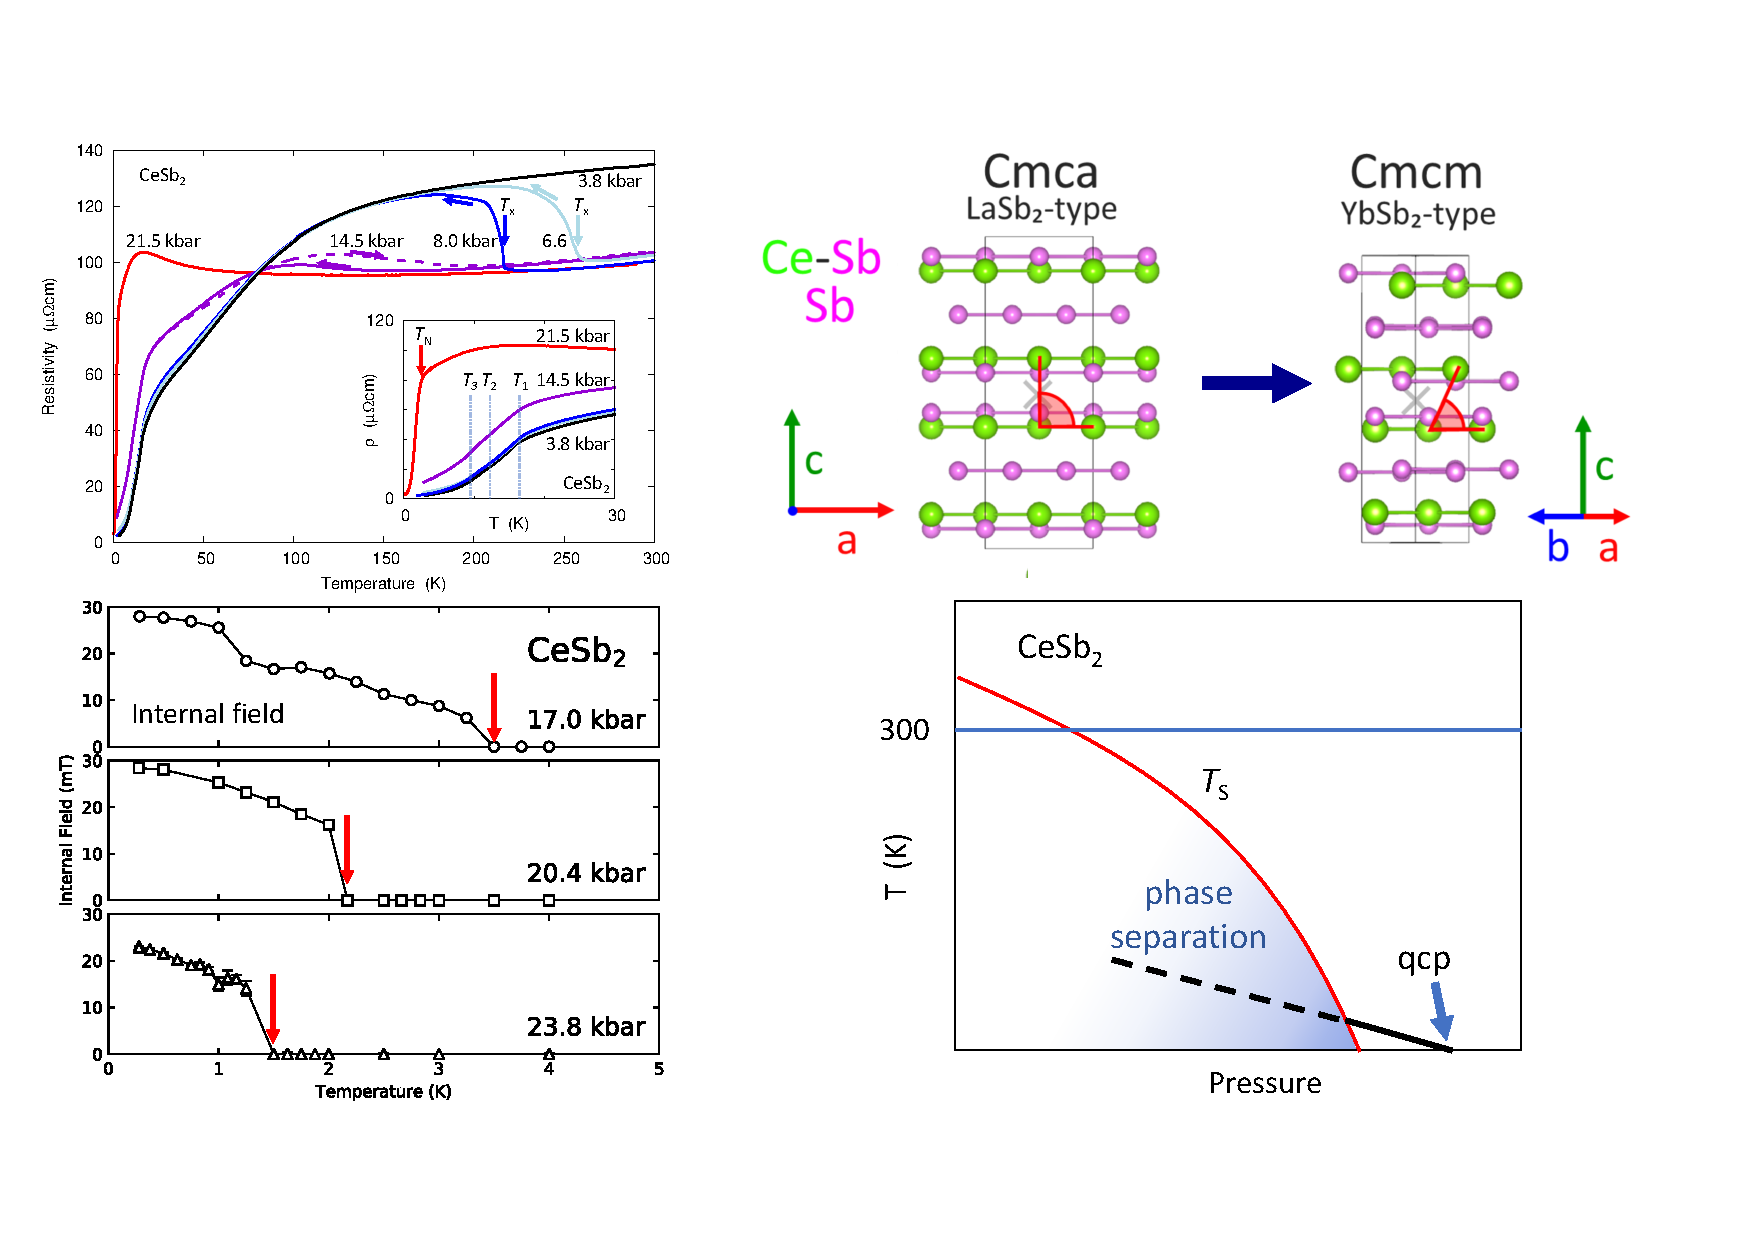
\includegraphics[width=1.2\columnwidth]{EndingPicture1}}
    %\vspace{-1em}
    %\begin{center}
    % Soft modes are built into some quasiperiodic structures. \\
      \mbox{\small Pressure-induced structural transition $\rightarrow$ correlated, magnetic high pressure state. }
    %\end{center}
    % \vspace*{\fill}
    % \centerline{\makebox[\linewidth]{\rule{0.85\textwidth}{0.4pt}}}
    % \centerline{\scriptsize P. Brown Sci. Adv. (2018)}
\end{frame}
    

    


%%% Local Variables: 
%%% mode: latex
%%% TeX-master: "GroTalk.tex"
%%% End: 
